\clearpage
%\quad
%\vspace{2cm}

\section{\textsl{Electronic background sketch}}
 \addtocontents{toc}{\smallskip \hspace{\parindent} [ \ref{k540v1} -- \ref{k540v2} -- \ref{k540v3} -- \ref{scp} ]  \par}

\label{imp1}
%\addcontentsline{toc}{chapter}{Proposition 1 -- \textsl{Electronic background sketch}}

\bigskip

The electronic background consists to realize a formal and structural direction according to some algorithmic process managed with a SuperCollider code. The material is computed in Common Lisp using the library \textsl{cl-gsa} from samples and/or scores (shortly this consists to `transpose' a given melody to a weighted tone).

Then the direction consists to determinate the duration of transformation between two events. An event is a combinatorics %(or not)
 -- see  algorithm \ref{ocwr} $\sim$\textsc{ocwr} and \textsc{ocwr} box description -- of frequential profiles. These combinatorics is included as set inside a combination called \texttt{symmetric-permutation} from the library \textsl{cl-cycle}. Each frequential profile is determined by an array of frequencies (as peaks), a respective array of amplitudes and a respective array of bandwidths (interpreted as grain) plus a resonant filter. This last is divided in 3 bandwidths which is correlated in temporal directivity to the three first formants and their respective bandwidths and intensity from Praat analysis of the recorded voices according to an appropriate concatenation. This last is scaled in order to match the total duration of the score.

\bigskip

The transformation --  that I call `peak morphing' -- consists to a linear interpolation between 2 points whose match a minimal distance.

\begin{figure}[h]
\begin{center}
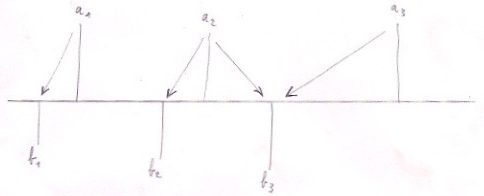
\includegraphics[scale=0.6]{img/9873}
\caption{Peak morphing from $a$ to $b$.}
\label{a1}
\end{center}
\end{figure}

$a_1 \rightarrow b_1, a_2 \rightarrow (b_2, b_3), a_3 \rightarrow b_3$

\smallskip

\begin{algorithm}
\caption{$\sim$\textsc{ocwr}$\,(list\,|\,R, dec)$}\label{ocwr}
\begin{algorithmic}%[1]

\State{/* \textsc{ocwr} for Ordered Combination Without Repetition */}

\If {$list \neq nil$}

$R=$[ $list$ ]

$dec=| list |$
\EndIf

\If {$dec=1$}

\Return $R$
\Else

\For {$item$ in $R$}

\If {$| item |=dec$}

\For {$position$ from $0$ to $| item |-1$}

$R.add\,(\,item \backslash item\,[\,position\,]\,)$

\EndFor
\EndIf
\EndFor

$\sim$\textsc{ocwr}$\,(\,nil, R,  dec-1\,)$

\EndIf

\end{algorithmic}
\end{algorithm}

\bigskip

The formal direction can be determined in terms of spatialisation, with $x$ as left/right axis, $y$ as front/back axis and $z$ as distance axis. The latter (see appendice \fullref{dist}) will determinate the presence level (or conversely the absence of sound depending on the audibility threshold).
These coordinate will be effective inside the total duration $D$ by a successive transformation duration $d$ according to the equality $D=\displaystyle \sum\limits_{i=1}^{\lambda}d_i$
$\;$ with $\lambda = card(\mathcal{C}_n)$ where $n=$ the number of synthesis and $\mathcal{C}_n$ the set of combinatorics with $n$ synthesis. 

Note that for  $\mathcal{C}_n=\{ C_1, C_2, \dots, C_{\lambda} \}$ the 'peak morphing' duration $d_i$ will be define from $C_{i-1}$ to $C_{i}$. This means that we have to initiate the process with the combination $C_0$.

\titlebox{\textit{\textbf{OCWR description}}}{In other words the cardinal of \textsc{ocwr} is the number of $k$-combinations for all $k$ minus the empty set defined by:

$\quad \displaystyle \sum\limits_{0  \le k \le n} \binom{n}{k}=2^n$

 For instance with 3 elements there are 8 combinations (subsets) including the empty set: 
 
 $\quad |\{\{\};\{1\};\{2\};\{3\};\{1,2\};\{1,3\};\{2,3\};\{1,2,3\}\}|=2^3 = 8$
 
 Representing these subsets (in the same order) as base 2 numbers:
 
 $\quad 0 - 000$
 
 $\quad 1 - 001$
 
 $\quad 2 - 010$
 
 $\quad 3 - 100$
 
 $\quad 4 - 011$
 
 $\quad 5 - 101$
 
 $\quad 6 - 110$
 
 $\quad 7 - 111$
 
 % {\scriptsize \textit{Source}: \url{https://en.wikipedia.org/wiki/Combination\#Number\_of\_k-combinations\_for\_all\_k}}
  }
  
\bigskip

\begin{algorithm}
\caption{$\sim$\textsc{peakMorphing}$\,(A, \,B )$}\label{pm}
\begin{algorithmic}%[1]

\State \textbf{args}
\State $\qquad A=$ initial profile
\State $\qquad B=$ final profile

\State 
\State $result=[\:]$

\For {$a$ in $A$}

$result.add\,(\,[\,a,\,nearest(B, a)\,]\,)$

\EndFor

\For {$b$ in $B$}

$result.add\,(\,[\,nearest(A, b),\,b\,]\,)$

\EndFor

\noindent \Return $result$

\end{algorithmic}
\end{algorithm}

Thus, the formal direction of each parameter will be defined by (i) determined functions (algorithms), (ii) stochastic distribution and (iii) according to the instrumental score; (i), (ii) and (iii) can be correlated and interdependent as $d=f(i)$ in terms of structural direction such as $\displaystyle \sum\limits_{i=1}^{\lambda}f(i)_i=D$.

\bigskip
In closing, let see the detailed procedure called initialisation for this soundscape. 

\begin{enumerate}
\label{m2tprecedure}
 \item Normalize the weighted profiles of the sample(s) and/or the score(s) generated by \texttt{m2tab} 
 %-- see the section instantiation in  \href{https://www.overleaf.com/read/sjhfhthgkgdj}{\textit{GSA: Melody to Tone}} -- 
 as an array.
  \item Determinate combination
  \begin{enumerate}
  \item Set the algoritm \ref{ocwr} $\sim$\textsc{ocwr} according to the number of weighted profiles.
 
  \item Compute symmetric permutation according to the length of \textsc{ocwr} regardless of $2^n-1$ (minus one excluding the empty set).
  
  For instance with $n=3$ as the number of profiles according to the point 1., the symmetric permutation takes as argument a random permutation or a deliberate permutation -- regarding the number of permutations for example -- of \texttt{(0 1 2 3 4 5 6)} for \texttt{lst} and for \texttt{code-lst}.
  \item Associate the combination of \textsc{ocwr} to the values of the flattened list of a symmetric permutation as indices applied to \textsc{ocwr}.
\end{enumerate}
\item Group the profile(s) according to the previous combination -- point 2.(c) -- as indices of the array of profiles.
\item Apply the algorithm \ref{pm} as a 'peak morphing' distribution between two successive events according to the sequence defined in point 3.
\item Set the durations transformation according to a deliberate shape.

For instance a sinusoid allows to stretch and to compress a sequence of durations like an elastic time line.
\item Allocate into buffers the formantic analysis -- see \nameref{fab} in appendice \fullref{fab} -- realized with some given recorded voice(s) as respectively the intensities, the three first formants and their associated bandwidths.
\end{enumerate}
Then, the sequence (3) is played with some resonant noise according to the frequencies as approximate rates, articulated with the 'peak morphing' (4) -- following the sequence of durations (5) -- and filtered according to some resonances set by the formants (6).

%==========================================================
%\clearpage
%\quad
%\vspace{2cm}

\section{\textsl{Proportional canon as an event climax}}
 \addtocontents{toc}{\smallskip \hspace{\parindent} [ \ref{cfso} -- \ref{tript} -- \ref{d01} -- \ref{scp} ]  \par}

\label{imp2}
%\addcontentsline{toc}{chapter}{Proposition 2 -- \textsl{Proportional canon as an event climax}}

Here are some introductory definitions:

\smallskip

\titlebox{\textit{\textbf{Proportional canon}}}
{The canon in music consists to repeat a melodic phrase -- or by extension a series of sound events -- according to various types of formal modalities in a contrapuntal relationship. One of them -- called proportional -- imitates the melodic line by changing the rhythmic values by increasing or decreasing in a proportional relationship, such as the resulting is a polyrhythm according to some factors of the initial tempo.}

\titlebox{\textit{\textbf{Event climax}}}
{A climax depicts a progression as an arsic movement followed most of the time by a thetic movement. This progression results in an increasing information flows -- may refer in this case to the density of events -- to a peak emphasizing the maximum intensity of the climax, and then might decrease in a release time logic.}
  
  \bigskip

 The construction of the initial rhythm can be intuitive (invention), referenced (quotation) and/or even created algorithmically. In the last case, it is possible to create rhythms with algorithmic processes such as those described with the libraries \textsl{cl-cycle}\footnote{The \textsl{cl-cycle} library is a set of algorithms that use the principle of cyclicality from a numerical sequence. The latter refers to an axiomatic symbolization by metaphorical transposition -- or other -- enabling the interpretation of a `mathematical reality' in a `musical reality' by correlation.} and \textsl{cl-gsa}\footnote{The \textsl{cl-gsa} library can be used to analyze and interpret a melody to create a weighted frequency profile correlated with the melody. However, these tools can be diverted to create rhythms from some relevant weights generated by the analysis.} inter alia.
  
\bigskip

\textbf{\textit{A}} - In order to realize the proportional canon as an event climax, we have to compute the durations and the delays of each voice according to a ratio $\rho$ as follow : according to the figure \ref{canon}, let $A$ be the first voice and $B$ the last voice, $d$ is the last delay in relation to the last voice such as:
  
\[
     d =
\begin{dcases}
	\frac{B}{2}  & \text{if } \tfrac{2}{3} \geqslant \rho > 0\\
	A \left ( 1+ \frac{3\rho}{2} \right )  & \text{if } \text{-} \tfrac{2}{3} \leqslant \rho < 0
   \end{dcases}
\]

  \noindent Thus, each intermediary voice will be a linear interpolation between the delays $0$ and $d$, and between the durations $A$ and $B$.
  
  Note that $\rho$ in order to be inside the longest duration (that is to say the first voice) has to be set between $-2/3$ and $2/3$ (zero excluded).
  
\begin{figure}[h]
\begin{center}
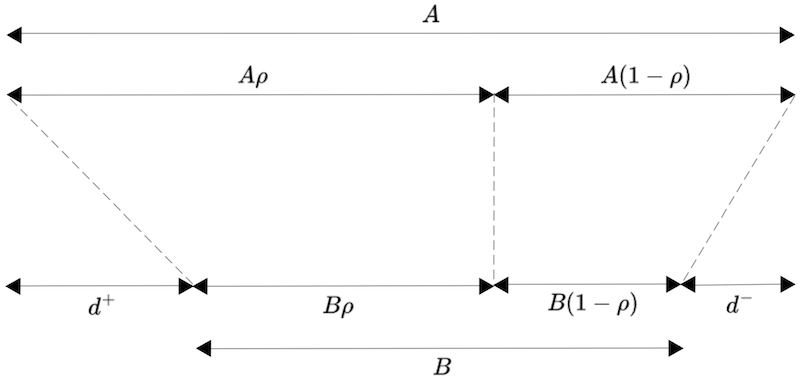
\includegraphics[scale=1.2]{img/3499}
\caption{Illustration of the proportional canon with $\rho = \varphi ^{-1}$ -- the Greek letter phi represents the golden ratio such as $\varphi = (1+ \sqrt 5)/2 \simeq 1.618$ -- according to the following equalities (knowing that $\rho$ is positive): $a_1m_a/ \varphi =m_aa_2$ and $ b_1m_b=m_bb_2=d=A/2 \varphi$.}
\label{canon}
\end{center}
\end{figure}
  
\textbf{\textit{B}} - Another way to realize the proportional canon is to apply the ratio $\rho$ for each voice according to a given duration for a given voice as follow: let $T$ be the set of $n$ durations (in other word $n$ is the number of voices) according to the ratio $\rho$ for a given duration $d_x$ of the $x^{th}$ voice, then

$T= \displaystyle \bigcup\limits_{i=1-x}^{n-x} d_x |\rho|^i\;$ with $0 < | \rho | \leqslant \frac{2}{3}$

\noindent and let $D$ be the set of the delays respectively assigned to $T$ according to the total duration $d_t$ such as

\[
     D =
\begin{dcases}
    0 \cup \displaystyle \bigcup\limits_{i=1}^{n-1} \sum\limits_{j=1}^i \frac{d_t \rho^j}{2} & \text{if }  \rho \text{ is positive }\\
    0 \cup \displaystyle \bigcup\limits_{i=1}^{n-1} \sum\limits_{j=0}^{i-1} d_t |\rho|^j \left ( 1+ \frac{3\rho}{2} \right )  & \text{if }  \rho \text{ is negative }
   \end{dcases}
\]

\begin{algorithm}[H]
\caption{$\sim$\textsc{proportionalCanon}$\,(n,\, d_x,\, \rho,\, x)$}\label{ldwd}
\begin{algorithmic}%[1]
\State \textbf{args}
\State $\qquad n =$ number of voices
\State $\qquad d_x =$ total duration or $x^{th}$ voice duration (if $x \neq nil$)
\State $\qquad \rho =$ ratio 
\State $\qquad x =$  $x^{th}$ voice with the duration $d_x$ (optional, note that if $x \neq nil$ this implies the algorithmic process described in \textbf{\textit{B}})
\State

\If{$x \in \mathbb{N}^{+*}$  \textbf{and} $x \leqslant n$}
\State
\State{/* algorithmic process \textbf{\textit{A}} */}

\State $d=nil$
\If{$ \rho > 0$}
\State $d=\rho /2$
\Else
\State $d=1+3 \rho /2$
\EndIf
\State $T =\:  n.interpolation[\,td, | td*\rho |\,]$
\State $D = \: n.interpolation[\,0, td*d\,]$
\State
\Return $(T, D)^T$
\State

\Else
\State{/* algorithmic process \textbf{\textit{B}} */}

\State $T=[\:]$
\State $i =1-x$
\While{$i=n-x$}

\State $T.add\left [d_x |\rho| ^i\right ]$

\State $i=i+1$
\EndWhile

\State
\State $D=[\,0\,]$
\For{$i$ from $1$ to $n-1$}
\If{$ \rho > 0$}

\State $D.add\left [ \sum_{j=1}^{i} d_t \rho^j /2 \right ]$
\Else

\State $D.add\left [ \sum_{j=0}^{i-1} d_t |\rho|^j \left (1+3\rho/2 \right ) \right ]$
\EndIf
\EndFor
\State
\Return $(T,D)^T$
\State{/* The result is a list of durations with delays. */}
\EndIf

\end{algorithmic}
\end{algorithm}

From here, it is possible to synchronize the result according to a minimal note length as duration. Then, let $C$ be the set of the durations of the canon (such as items of $C$ is the set of durations of $i$ voices) and $m$ the duration of the minimal value such as

\bigskip

$syncDur = \displaystyle \bigcup\limits_{i \in C} \bigcup\limits_{j \in i} \displaystyle \left [ \frac{j}{m} \right ] \cdot m$
 
\bigskip 
\bigskip
 
 A last word concerning the melody and the counterpoint. The melody -- or other as a \textit{klangfarbenmelodie} for instance -- can be considered according to some possible strategies.

The first one consists to attribute the same melody for each voice according their respective 'tempo'. In this case, the 'counterpoint' consists to adjust the ratio $\rho$.

The second one consists to manipulate the melody by transformation and/or by constraints -- or any kind of variation -- on the melody itself, or on the melodico-rhythmic resultant of the canon into a dialectic counterpoint. 

From here, we can add a third point in a way to consider only the rhythmic dimension. Like this, we are free to consider each voice independently of a predefined melody, on their own or in a holistic way.

Of course, all these points are empirical, but they can be integrated into a system of concepts.
For instance, the number of voices can be equal to the number of notes of a given chord, thus each voice plays a unique note respectively from the notes composing the aforesaid chord as a 'pedal note'.

%++++++++++++++++++++++++++++++++++++++++++++++++++++++++++
%\quad
%\vspace{2cm}

\section{\textsl{Fractal}}
 \addtocontents{toc}{\smallskip \hspace{\parindent} [ \ref{cfso} -- \ref{hex0} -- \ref{d01} -- \ref{105A1408} ]  \par}

\label{imp3}
%\addcontentsline{toc}{chapter}{Proposition 3 -- \textsl{Fractal}}

\begin{figure}[h]
\begin{center}
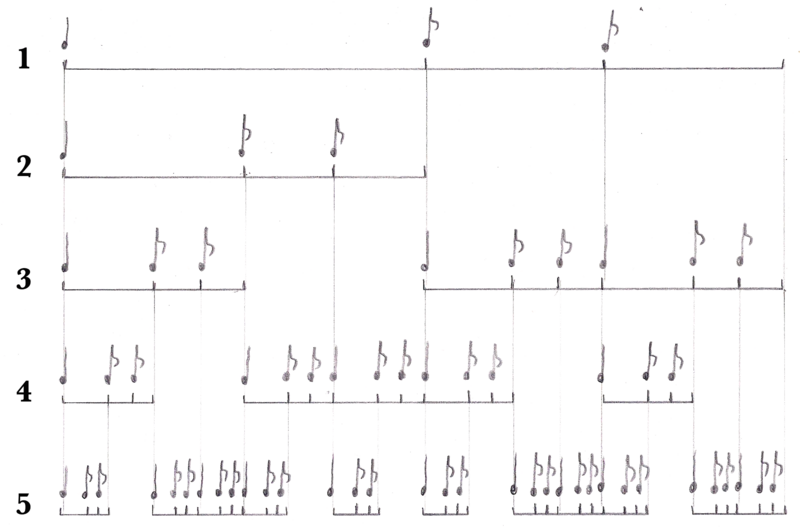
\includegraphics[scale=1.7]{img/1548}
\caption{Illustration of 5 levels of fractal recursivity from the rhythm: quarter note, eighth note, eighth note. In this case, each recursivity implies the doubling of the tempo.}
\label{fractal}
\end{center}
\end{figure}

\titlebox{\textit{\textbf{Fractal}}}
{A fractal is a natural phenomenon or a mathematical set that exhibits a repeating pattern that displays at every scale. It is also known as expanding symmetry or evolving symmetry. If the replication is exactly the same at every scale, it is called a self-similar pattern -- as showed on figure \ref{fractal}. 

%\scriptsize \textit{Source}: \url{https://en.wikipedia.org/wiki/Fractal}
 }

\begin{algorithm}[h]
\caption{$\sim$\textsc{fractal}$\,(rtm,\, dur,\, rec,\, min,\, al\,|\,R,\, int)$}\label{fra}
\begin{algorithmic}%[1]
\State \textbf{args}
\State $\qquad rtm =$ rhythm defined by a numerical array as a list of durations of  event.
\State $\qquad dur =$ total duration (mean to scale such as $\sum rtm = dur$).
\State $\qquad rec =$ number of dimensions or recursivity.
\State $\qquad min =$ minimal duration accepted.
\State $\qquad al =$ is a list of events according to $rtm$. If $al = nil$ then the new events according to the level of recursion, are defined as $1$, if not as $0$.
\State \textbf{args -- recursive call}
\State $\qquad R =$ temporary result.
\State $\qquad int =$ intermediate durations in relation with the number of recursivity.
\State

\State $tmpR=[\:]$
\If{$ rec=nil$} $rec=0$
\EndIf
\If{$ min=nil$} $min=0$
\EndIf
\If{$ R=nil$} $R=[rtm.as(\sum rtm=dur)]$
\EndIf
\If{$ int=nil$}
$int = assoc(rtm, al)$
\EndIf
\For{$i$ in $R[0]$}
\If{$ i=max(R[0])$} $tmpR.add[rtm.as(\sum rtm=i)]$
\Else $\: tmpR.add[[i]]$
\EndIf
\EndFor

\State
\If{$rec=0$ \textbf{or} $min \geqslant min(R[0])$}

\Return $[R,int]$
\Else

\State $idr=[\:]$
\For{$item$ in $R[0]$ \textbf{and} $position$ from $0$ to $| R[0] |-1$}
\State $idrn=[\:]$
\Repeat $\;idrn.add[item]$ 
\Until $| tmpR[position] |$
\State $idr.add[idrn]$
\EndFor
\State $\sim$\textsc{fractal}($rtm, dur, rec-1, min, al, \newline
        \hspace*{15em} R.add[\bigcup tmpR], int.add[\bigcup assoc(idr, al)]$)

\EndIf

\end{algorithmic}
\end{algorithm}

The fractal recursivity stops when the number of recursivity $rec$ is reached, unless the minimal duration defined with $min$ (meaning $min \ne$ nil) is reached before. For instance, figure \ref{fractal} could be parametrised with $rec=5$ or $min$ equal to the value of the shortest eighth note recognized on level 5. 

This kind of fractality describes a process from a final duration into `inferior' dimension according to the maximal differential duration for each recursivity.  

  \smallskip
 Here are some precisions concerning the algorithm \ref{fractal} $\sim$\textsc{fractal} such as the arguments and the output result.
 
\begin{itemize}[label=\textbullet]
\item The algorithm takes as arguments
\begin{itemize}[label=$\rightarrow$]
\item  the initial rhythm \texttt{RTM}, 
 \item the total duration \texttt{DUR},
 \item  and the number of recursivity \texttt{REC} \underline{or} the \hbox{lowest} allowed duration, involving a variable number of recursivity, such as \texttt{REC = RES[i].size}, with \texttt{RES} as the resulting array, 
 \item and optionally \texttt{AL} (see next point). 
 \end{itemize}
\item The \texttt{RES[1]} is a list of events -- for instance, each event can be defined by the command line \textsl{enkode}
%\footnote{See \href{https://www.overleaf.com/read/sjhfhthgkgdj}{\textit{GSA: Documentation of the executable script \textsl{enkode}}}.}
 -- according to the \texttt{RTM} defined by the option \texttt{AL}. If \texttt{AL = nil} then the new events according to the level of recursion, are defined as $1$, if not as $0$.
\item For $n$ from \texttt{0} to \texttt{REC$-1$};
\begin{itemize}[label=$\rightarrow$]
\item \texttt{RES[0][$n$].size = RES[1][$n$].size}
\item $\sum$ \texttt{RES[0][}$n$\texttt{] =  DUR}
\end{itemize}
\item \texttt{RES[i][j].size$-1$} is a multiple of \texttt{RTM.size$-1$}.

\item \texttt{RES[0][0]} is the last recursion, as an array of all events duration of the whole sequence.

\end{itemize}

\section{Discussion}
\label{Discussion}
%\addcontentsline{toc}{chapter}{\nameref{Discussion}}

\titlebox{\textit{\textbf{Last but not least}}}
{Now, the art -- if I may use that word -- should be to establish a relationship between each element of the system as a formal object inside the morphological context predefined or emergent.

This implies a metaphysical order relationship between the formal inference system and the artistic intent.}

\titlebox{\textit{\textbf{A philosophical point}}}
{The initial material, here we are talking about a sample as a sound file or a partition, convey its own immanence according to the developmental process implementation. I do make a link between the transcendence of the process and the immanence of the initial component(s). Thus, the result is an emergent form, which can be determinist or indeterminist in chaotic terms \citep{tdc} depending on the case therefore sensitive to initial conditions.}